\documentclass{standalone}
\usepackage{tikz}
\usetikzlibrary{patterns, positioning}


\begin{document}
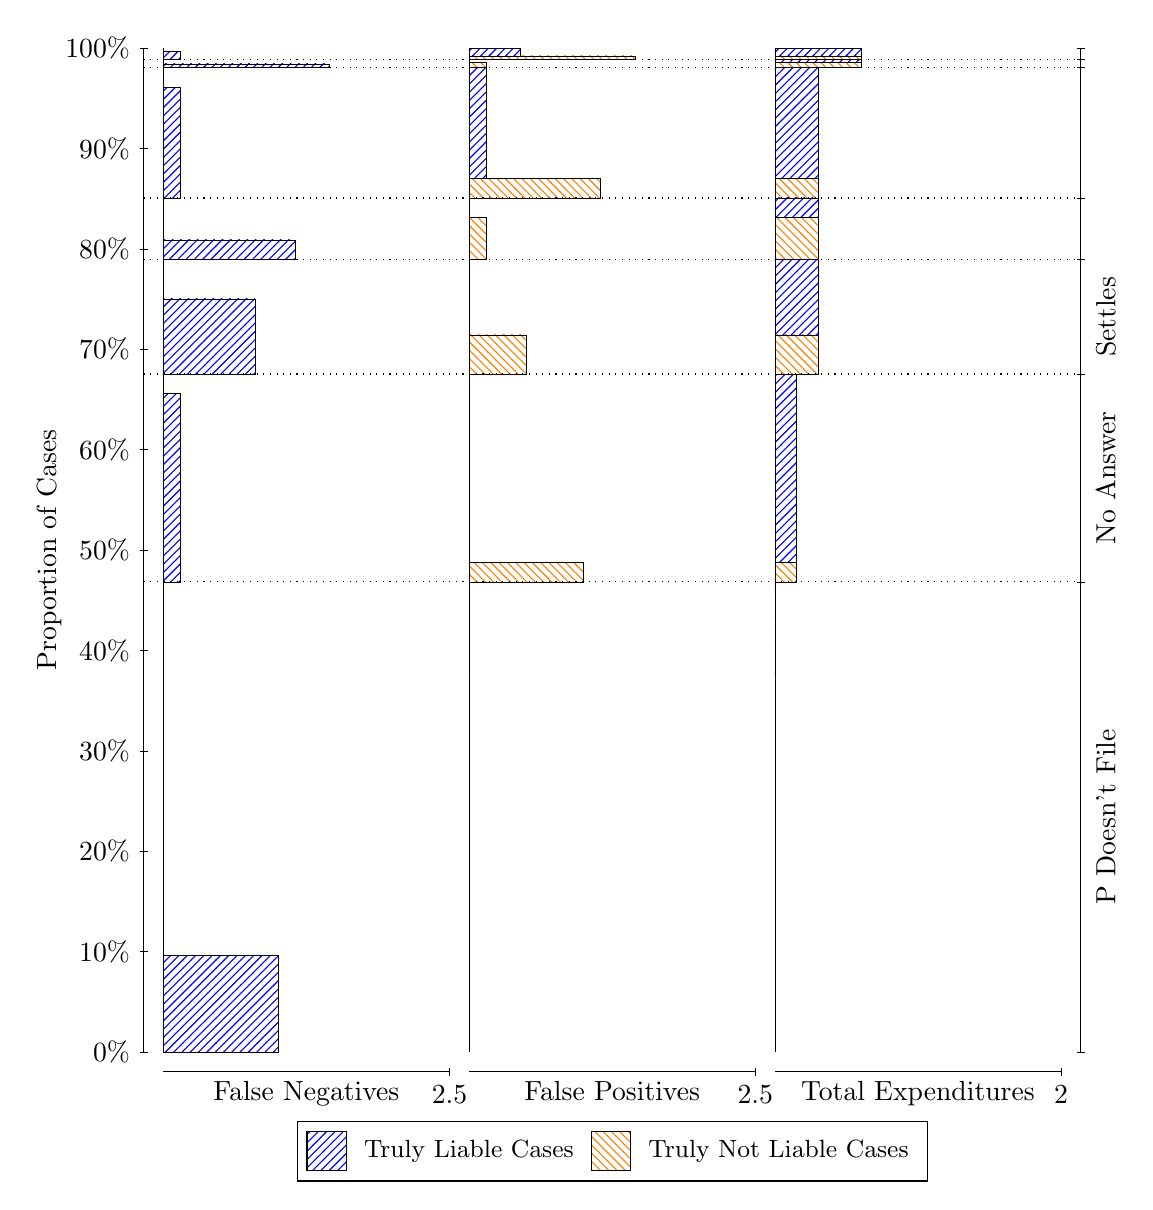
\begin{tikzpicture}
\draw[black, very thin] (1.5,1.75) -- (1.5,14.5);
\node[rotate=90, text=black, anchor=center] at (0.3, 8.125) {Proportion of Cases};
\draw[black, very thin] (1.45,1.75) -- (1.55,1.75);
\node[text=black, anchor=east] at (1.45, 1.75) {0\%};
\draw[black, very thin] (1.45,3.025) -- (1.55,3.025);
\node[text=black, anchor=east] at (1.45, 3.025) {10\%};
\draw[black, very thin] (1.45,4.3) -- (1.55,4.3);
\node[text=black, anchor=east] at (1.45, 4.3) {20\%};
\draw[black, very thin] (1.45,5.575) -- (1.55,5.575);
\node[text=black, anchor=east] at (1.45, 5.575) {30\%};
\draw[black, very thin] (1.45,6.85) -- (1.55,6.85);
\node[text=black, anchor=east] at (1.45, 6.85) {40\%};
\draw[black, very thin] (1.45,8.125) -- (1.55,8.125);
\node[text=black, anchor=east] at (1.45, 8.125) {50\%};
\draw[black, very thin] (1.45,9.4) -- (1.55,9.4);
\node[text=black, anchor=east] at (1.45, 9.4) {60\%};
\draw[black, very thin] (1.45,10.675) -- (1.55,10.675);
\node[text=black, anchor=east] at (1.45, 10.675) {70\%};
\draw[black, very thin] (1.45,11.95) -- (1.55,11.95);
\node[text=black, anchor=east] at (1.45, 11.95) {80\%};
\draw[black, very thin] (1.45,13.225) -- (1.55,13.225);
\node[text=black, anchor=east] at (1.45, 13.225) {90\%};
\draw[black, very thin] (1.45,14.5) -- (1.55,14.5);
\node[text=black, anchor=east] at (1.45, 14.5) {100\%};

\draw[black, very thin] (13.4,1.75) -- (13.4,14.5);
\draw[black, very thin] (13.35,1.75) -- (13.45,1.75);
\node[anchor=west] at (13.35, 1.75) {};
\draw[black, very thin] (13.35,7.7207) -- (13.45,7.7207);
\node[anchor=west] at (13.35, 7.7207) {};
\draw[black, very thin] (13.35,10.36) -- (13.45,10.36);
\node[anchor=west] at (13.35, 10.36) {};
\draw[black, very thin] (13.35,11.811) -- (13.45,11.811);
\node[anchor=west] at (13.35, 11.811) {};
\draw[black, very thin] (13.35,12.596) -- (13.45,12.596);
\node[anchor=west] at (13.35, 12.596) {};
\draw[black, very thin] (13.35,14.256) -- (13.45,14.256);
\node[anchor=west] at (13.35, 14.256) {};
\draw[black, very thin] (13.35,14.358) -- (13.45,14.358);
\node[anchor=west] at (13.35, 14.358) {};
\draw[black, very thin] (13.35,14.5) -- (13.45,14.5);
\node[anchor=west] at (13.35, 14.5) {};

\draw[black, very thin, pattern color=blue, pattern=north east lines] (1.75,1.75) rectangle (3.2033,2.9752);
\draw[black, very thin, pattern color=orange, pattern=north west lines] (1.75,2.9752) rectangle (1.75,7.7207);
\draw[black, very thin, pattern color=blue, pattern=north east lines] (1.75,7.7207) rectangle (1.968,10.115);
\draw[black, very thin, pattern color=orange, pattern=north west lines] (1.75,10.115) rectangle (1.75,10.36);
\draw[black, very thin, pattern color=blue, pattern=north east lines] (1.75,10.36) rectangle (2.9127,11.314);
\draw[black, very thin, pattern color=orange, pattern=north west lines] (1.75,11.314) rectangle (1.75,11.811);
\draw[black, very thin, pattern color=blue, pattern=north east lines] (1.75,11.811) rectangle (3.4213,12.062);
\draw[black, very thin, pattern color=orange, pattern=north west lines] (1.75,12.062) rectangle (1.75,12.596);
\draw[black, very thin, pattern color=blue, pattern=north east lines] (1.75,12.596) rectangle (1.968,14.004);
\draw[black, very thin, pattern color=orange, pattern=north west lines] (1.75,14.004) rectangle (1.75,14.256);
\draw[black, very thin, pattern color=blue, pattern=north east lines] (1.75,14.256) rectangle (3.8573,14.299);
\draw[black, very thin, pattern color=orange, pattern=north west lines] (1.75,14.299) rectangle (1.75,14.358);
\draw[black, very thin, pattern color=blue, pattern=north east lines] (1.75,14.358) rectangle (1.968,14.458);
\draw[black, very thin, pattern color=orange, pattern=north west lines] (1.75,14.458) rectangle (1.75,14.5);
\draw[black, very thin, pattern color=orange, pattern=north west lines] (5.6333,1.75) rectangle (5.6333,6.4955);
\draw[black, very thin, pattern color=blue, pattern=north east lines] (5.6333,6.4955) rectangle (5.6333,7.7207);
\draw[black, very thin, pattern color=orange, pattern=north west lines] (5.6333,7.7207) rectangle (7.0867,7.9655);
\draw[black, very thin, pattern color=blue, pattern=north east lines] (5.6333,7.9655) rectangle (5.6333,10.36);
\draw[black, very thin, pattern color=orange, pattern=north west lines] (5.6333,10.36) rectangle (6.36,10.857);
\draw[black, very thin, pattern color=blue, pattern=north east lines] (5.6333,10.857) rectangle (5.6333,11.811);
\draw[black, very thin, pattern color=orange, pattern=north west lines] (5.6333,11.811) rectangle (5.8513,12.345);
\draw[black, very thin, pattern color=blue, pattern=north east lines] (5.6333,12.345) rectangle (5.6333,12.596);
\draw[black, very thin, pattern color=orange, pattern=north west lines] (5.6333,12.596) rectangle (7.3047,12.848);
\draw[black, very thin, pattern color=blue, pattern=north east lines] (5.6333,12.848) rectangle (5.8513,14.256);
\draw[black, very thin, pattern color=orange, pattern=north west lines] (5.6333,14.256) rectangle (5.8513,14.315);
\draw[black, very thin, pattern color=blue, pattern=north east lines] (5.6333,14.315) rectangle (5.6333,14.358);
\draw[black, very thin, pattern color=orange, pattern=north west lines] (5.6333,14.358) rectangle (7.7407,14.4);
\draw[black, very thin, pattern color=blue, pattern=north east lines] (5.6333,14.4) rectangle (6.2873,14.5);
\draw[black, very thin, pattern color=orange, pattern=north west lines] (9.5167,1.75) rectangle (9.5167,6.4955);
\draw[black, very thin, pattern color=blue, pattern=north east lines] (9.5167,6.4955) rectangle (9.5167,7.7207);
\draw[black, very thin, pattern color=orange, pattern=north west lines] (9.5167,7.7207) rectangle (9.7892,7.9655);
\draw[black, very thin, pattern color=blue, pattern=north east lines] (9.5167,7.9655) rectangle (9.7892,10.36);
\draw[black, very thin, pattern color=orange, pattern=north west lines] (9.5167,10.36) rectangle (10.062,10.857);
\draw[black, very thin, pattern color=blue, pattern=north east lines] (9.5167,10.857) rectangle (10.062,11.811);
\draw[black, very thin, pattern color=orange, pattern=north west lines] (9.5167,11.811) rectangle (10.062,12.345);
\draw[black, very thin, pattern color=blue, pattern=north east lines] (9.5167,12.345) rectangle (10.062,12.596);
\draw[black, very thin, pattern color=orange, pattern=north west lines] (9.5167,12.596) rectangle (10.062,12.848);
\draw[black, very thin, pattern color=blue, pattern=north east lines] (9.5167,12.848) rectangle (10.062,14.256);
\draw[black, very thin, pattern color=orange, pattern=north west lines] (9.5167,14.256) rectangle (10.607,14.315);
\draw[black, very thin, pattern color=blue, pattern=north east lines] (9.5167,14.315) rectangle (10.607,14.358);
\draw[black, very thin, pattern color=orange, pattern=north west lines] (9.5167,14.358) rectangle (10.607,14.4);
\draw[black, very thin, pattern color=blue, pattern=north east lines] (9.5167,14.4) rectangle (10.607,14.5);
\draw[black, dotted] (1.5,7.7207) -- (13.4,7.7207);
\draw[black, dotted] (1.5,10.36) -- (13.4,10.36);
\draw[black, dotted] (1.5,11.811) -- (13.4,11.811);
\draw[black, dotted] (1.5,12.596) -- (13.4,12.596);
\draw[black, dotted] (1.5,14.256) -- (13.4,14.256);
\draw[black, dotted] (1.5,14.358) -- (13.4,14.358);
\draw[black, very thin] (1.75,1.5) -- (5.3833,1.5);
\node[text=black, anchor=north] at (3.5667, 1.5) {False Negatives};
\draw[black, very thin] (5.3833,1.45) -- (5.3833,1.55);
\node[text=black, anchor=north] at (5.3833, 1.45) {2.5};

\draw[black, very thin] (5.6333,1.5) -- (9.2667,1.5);
\node[text=black, anchor=north] at (7.45, 1.5) {False Positives};
\draw[black, very thin] (9.2667,1.45) -- (9.2667,1.55);
\node[text=black, anchor=north] at (9.2667, 1.45) {2.5};

\draw[black, very thin] (9.5167,1.5) -- (13.15,1.5);
\node[text=black, anchor=north] at (11.333, 1.5) {Total Expenditures};
\draw[black, very thin] (13.15,1.45) -- (13.15,1.55);
\node[text=black, anchor=north] at (13.15, 1.45) {2};

\node[text=black, centered, rotate=90] at (13.72, 4.7354) {P Doesn't File};
\node[text=black, centered, rotate=90] at (13.72, 9.0402) {No Answer};
\node[text=black, centered, rotate=90] at (13.72, 11.085) {Settles};





\draw (7.449999999999999,1.5) node[draw=none] (baseCoordinate) {};
\begin{scope}[align=center]
        \matrix[scale=0.5, draw=black, below=0.5cm of baseCoordinate, nodes={draw}, column sep=0.1cm]{
            \node[rectangle, draw, minimum width=0.5cm, minimum height=0.5cm, pattern color=blue, pattern=north east lines] {}; &
            \node[draw=none, font=\small, text=black] (B) {Truly Liable Cases}; &
            \node[rectangle, draw, minimum width=0.5cm, minimum height=0.5cm, pattern color=orange, pattern=north west lines] {}; &
            \node[draw=none, font=\small, text=black] (B) {Truly Not Liable Cases}; \\
            };
\end{scope}

\end{tikzpicture}
\end{document}